% \RequirePackage[l2tabu, orthodox]{nag}
% \documentclass{article}

% % FONTS
\usepackage[T1]{fontenc}

% Replace default Latin Modern typewriter with its proportional counterpart
% http://www.tug.dk/FontCatalogue/lmoderntypewriterprop/
\renewcommand*\ttdefault{lmvtt}

%\usepackage[bitstream-charter]{mathdesign} % not needed for mtpro
\usepackage{amsmath}
\usepackage[subscriptcorrection,
            amssymbols,
            mtpbb,
            mtpcal,
            nofontinfo  % suppresses all warnings
           ]{mtpro2} %TODO: put htis back in and take out mathdesign
\usepackage{scalefnt,letltxmacro}
\LetLtxMacro{\oldtextsc}{\textsc}
\renewcommand{\textsc}[1]{\oldtextsc{\scalefont{1.10}#1}}
\usepackage[scaled=0.92]{PTSans}


% % COLOR
\usepackage[usenames,dvipsnames]{xcolor}
\definecolor{Green}{HTML}{156946}

% % SPACING and TEXT
\usepackage[final,expansion=alltext]{microtype}
\usepackage[english]{babel}
\usepackage{afterpage}
\usepackage{framed}


% define a paragraph header function
\DeclareRobustCommand{\parhead}[1]{\textbf{#1}~}

% % EDITING
% paragraph helper
\DeclareRobustCommand{\PP}{\textcolor{Plum}{\P} }

% % COUNTERS
\usepackage{enumitem}
\renewcommand{\labelenumi}{\color{black!67}{\arabic{enumi}.}}
\renewcommand{\labelenumii}{{\color{black!67}(\alph{enumii})}}
\renewcommand{\labelitemi}{{\color{black!67}\tiny$\blacksquare$}}
\renewcommand{\labelitemii}{{\color{black!67}\textbullet}}
\renewcommand{\labelitemiii}{{\color{black!67}\scriptsize$\blacktriangleright$}}

% FIGURES
\usepackage{graphicx}

% TABLES
\usepackage{booktabs}

% ALGORITHMS
\usepackage[algoruled]{algorithm2e}
\usepackage{listings}
\usepackage{fancyvrb}
\fvset{fontsize=\normalsize}

% % HYPERREF
\usepackage[colorlinks,linktoc=all]{hyperref} %TODO: rm draft
\usepackage[all]{hypcap}
\hypersetup{citecolor=Green}
\hypersetup{linkcolor=Green}
\hypersetup{urlcolor=Green}

% % CLEVEREF must come after HYPERREF
\usepackage[nameinlink]{cleveref}

% BIBLIOGRPHY: get rid of reference labels
\makeatletter
	\renewcommand\@biblabel[1]{}
\makeatother

% ACRONYMS
\usepackage[acronym,smallcaps,nowarn]{glossaries}
% \makeglossaries

% % COLOR DEFINITIONS
\newcommand{\green}[1]{\textcolor{Green}{#1}}


% LISTINGS DEFINTIONS
\lstdefinestyle{mystyle}{
    commentstyle=\color{Green},
    keywordstyle=\color{Green},
    numberstyle=\tiny\color{black!60},
    stringstyle=\color{Green},
    basicstyle=\ttfamily,
    breakatwhitespace=false,
    breaklines=true,
    captionpos=b,
    keepspaces=true,
    numbers=left,
    numbersep=5pt,
    showspaces=false,
    showstringspaces=false,
    showtabs=false,
    tabsize=2
}
\lstset{style=mystyle}

% ALGORITHMS
\usepackage[algoruled]{algorithm2e}

% FRAMES
\usepackage[linewidth=1pt]{mdframed}
\DeclareRobustCommand{\mb}[1]{\ensuremath{\boldsymbol{\mathbf{#1}}}}

\DeclareMathOperator*{\argmax}{arg\,max}
\DeclareMathOperator*{\argmin}{arg\,min}

\DeclareRobustCommand{\KL}[2]{\ensuremath{\textrm{KL}\left(#1\;\|\;#2\right)}}

\newcommand{\mbx}{\mathbold{x}}
\newcommand{\mbX}{\mbf{X}}

\newcommand{\mbz}{\mathbold{z}}

\newcommand{\mbI}{\mbf{I}}

\newcommand{\mbZ}{\mbf{Z}}
\newcommand{\mbL}{\mbf{L}}

\newcommand{\mbtheta}{\mathbold{\theta}}
\newcommand{\mbTheta}{\mathbold{\Theta}}
\newcommand{\mbomega}{\mathbold{\omega}}
\newcommand{\mbOmega}{\mathbold{\Omega}}
\newcommand{\mbsigma}{\mathbold{\sigma}}
\newcommand{\mbSigma}{\mathbold{\Sigma}}

\newcommand{\mblambda}{\mathbold{\lambda}}
\newcommand{\mbgamma}{\mathbold{\gamma}}
\newcommand{\mbzeta}{\mathbold{\zeta}}
\newcommand{\mbeta}{\mathbold{\eta}}
\newcommand{\mbbeta}{\mathbold{\beta}}
\newcommand{\mbphi}{\mathbold{\phi}}
\newcommand{\mbmu}{\mathbold{\mu}}
\newcommand{\mbrho}{\mathbold{\rho}}

\newcommand\dif{\mathop{}\!\mathrm{d}}
\newcommand{\diag}{\textrm{diag}}
\newcommand{\supp}{\textrm{supp}}

\newcommand{\E}{\mathbb{E}}
\newcommand{\Var}{\mathbb{V}\textrm{ar}}

\newcommand{\bbN}{\mathbb{N}}
\newcommand{\bbZ}{\mathbb{Z}}
\newcommand{\bbR}{\mathbb{R}}
\newcommand{\bbS}{\mathbb{S}}

\newcommand{\cL}{\mathcal{L}}

\newcommand{\cN}{\mathcal{N}}
\newcommand{\Gam}{\textrm{Gam}}
\newcommand{\InvGam}{\textrm{InvGam}}

\newcommand{\g}{~\vert~}
\newacronym{KL}{kl}{Kullback-Leibler}
\newacronym{ELBO}{elbo}{\emph{evidence lower bound}}
\newacronym{POPELBO}{pop-elbo}{\emph{population evidence lower bound}}

\newacronym{SVI}{svi}{stochastic variational inference}
\newacronym{BUMPVI}{bump-vi}{bumping variational inference}

\newacronym{GMM}{gmm}{Gaussian mixture model}
\newacronym{LDA}{lda}{latent Dirichlet allocation}

\newacronym{SUTVA}{sutva}{stable unit treatment value assumption}

% fanciness for quote
\usepackage{epigraph}
\patchcmd{\epigraph}{\@epitext{#1}}{\itshape\@epitext{#1}}{}{}

\begin{document}

\title{Who, What, When, Where, and Why? \\ A Computational Approach to Understanding Historical Events Using State Department Cables}

\author{Allison J.B. Chaney, Hanna Wallach, David M. Blei}

\maketitle

\vspace{0.3in}

\begin{center}
\parbox{3.5in}{
\raggedright{
 	\emph{We can do nothing but scrutinize historical events themselves if we want to discover what they are.}}\\
\smallskip
\raggedleft{-- Dean W.R. Matthews, \emph{What is an Historical Event?}}
}
\end{center}

\vspace{0.5in}

\begin{abstract}
	We develop computational methods for analyzing historical documents to identify events of potential historical significance. Significant events are characterized by interactions between entities (e.g., countries, organizations, individuals) that deviate from typical interaction patterns. When studying historical events, historians and political scientists commonly read large quantities of text to construct an accurate picture of who, what, when, and where---a necessary precursor to answering the more nuanced question, ``Why?'' Our methods help historians identify possible events from the texts of historical communication. Specifically, we build on topic modeling to distinguish between topics that describe ``business-as-usual'' and topics that deviate from these patterns, where deviations are also indicated by particular entities interacting during particular periods of time. To demonstrate our methods, we analyze a corpus of 2 million State Department cables from 1973 to 1977.  For example, we show that we are able to detect and characterize the Fall of Saigon.
\end{abstract}


\section{Introduction}

Communications between the U.S. State Department and its embassies have historically been called \emph{diplomatic cables}, derived from the time when physical cables were used for such communications.
We obtained around two million of these cables sent between 1973 and 1977 via the History Lab at Columbia,\footnote{http://history-lab.org} which received them from the Central Foreign Policy Files at the National Archives.  In addition to the text of the cables themselves, each document is supplemented with information about who sent the cable (e.g., the State Department, the U.S. Embassy in Saigon, or an individual by name), who received the message (often multiple entities), and the date the message was sent.
Excerpts from three example cables are shown in Figure~\ref{fig:cables_example}.

\begin{figure}[ht]
\centering
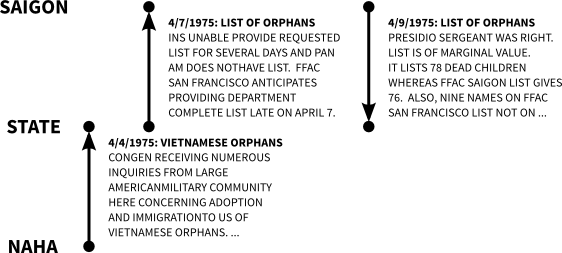
\includegraphics[width=\textwidth]{fig/cables_orphan_example.png}
\caption{Example excerpts of cables sent in April 1975 concerning orphans from the Vietnam War.}
\label{fig:cables_example}
\end{figure}

Historians and political scientists are interested in the process of sending cables---of particular interest is identifying historical events from a collection of these cables.  These experts want to know \emph{when} events happen, as well as \emph{what} happens during the event, which includes the parties sending and receiving messages (\emph{who}) and \emph{where} the event is located. 

For this work, we characterize an event in two ways: \emph{when} it occurs and \emph{what} occurs.  We assume that only one event can begin on any given day, which allows us to describe each day in terms of the probability of an event starting that day.  We can also assume that an event will influence cables for a set time period after it starts---this way, we only need to discover the starting day for each event.  
To understand \emph{what} occurs, we can summarize the cable message content with a topic model such as LDA~\citep{Blei:2003} and model event content in that same space.


\section{A Generative Model of Events}
Our model is a generative process---we make assumptions about how the data came to be and describe these assumptions in terms of probability distributions.  Given our model and observed data, the task is then to reverse the generative process to find the hidden quantities that (retrospectively) generated the data.

Consider an entity like the Bangkok American embassy.  We can imagine that there is a stream of cables being sent by this embassy---some might be sent to the US State Department, others to another American embassy like Hong Kong, and perhaps a few are sent to individuals by name.  Each of these cables has an associated send date, and we can represent the content of the cable with a topic model; we call these cable descriptions $\theta$, which is a matrix of $D$ cables (or documents) by $K$ topics.\footnote{This allows us to represent the cable in terms of about 100 topics rather than in terms of hundreds of thousands of vocabulary words. We can discover these topics with LDA and treat them as fixed observations going forward.}

An entity will usually talk about certain topics and with certain frequency. The Bangkok embassy, for instance, sent and average of 22 cables per day in the 1970s, and was concerned with topics regarding southeast Asia more generally.  We can describe the general interests of entities in the same topic space we use to describe individual cables and we will call these per-entity interests $\phi$ and can assign them a formal distribution.
\begin{itemize}
\item Draw the entity's base topics: $\phi_{0k} \sim \mbox{Gamma}(\alpha, \beta)$
\end{itemize}
Eventually we will want to model the interactions between entities, but for now we can consider a single entity at a time.

Now imagine that at a particular time, an event occurs, such as the capture of Saigon during the Vietnam war.  We do not directly observe that events occurs, but each event can again be described in the same topic space used to describe individual cables.  Whether or not an event occurs at a particular time step is represented by $\epsilon_t$ and the content of the event (or its topical representation) is called $\pi_t$.

\begin{itemize}
\item For each day $i$ with date $a_i$:
\begin{itemize}
\item Generate event occurrence/strength $\epsilon \sim \mbox{Poisson}
(\eta_\epsilon)$,\footnote{Event occurrence can alternatively be modeled with a Bernoulli distribution.  The advantage to the Bernoulli is that it is more interpretable.  Poisson-distributed event occurrences lay the groundwork for more complicated models based in Poisson processes, and allow for a nuanced interpretation of multiple real-world events occurring in a single day, but convolving into a single event in model space.} where $\eta_\epsilon$ is a fixed, non-negative
hyperparameter for the mean event strength.
\item Generate the day/event's description in terms of each topic $k$: $\pi_{ik} \sim \mbox{Gamma}(\alpha_0, \beta_0)$, where $\alpha_0$ and $\beta_0$ are fixed hyperparameters.
\end{itemize}
\end{itemize}

When an event occurs, both the frequency of cables being sent and the cable content changes. The Bangkok embassy sent 31 cables the day following the capture of Saigon (a 36\% increase over the average), and the majority of these cables are about Vietnam war refugees.  Thus we imagine that an entity's stream of cables is controlled by what it usually talks about (and how often) as well as the higher level stream of unobserved events.  The influence of an event does not last indefinitely, however, so we model the decay of its magnitude with some function $f$.
While many decay functions can be used, we define the event decay function to be a simple linear decrease: \[f(a, c) =
\begin{cases}
	1 - \frac{c-a}{d}, & \mbox{if } a \le c < a+d \\
	0, & \mbox{otherwise,}
\end{cases} \]
where $d$ is the time distance (in days) after event $a$ at which point the event is no longer relevant.

When we analyze the cables with this model setup, we disentangle cables that represent ``business as usual'' from those that reflect the higher-order event stream.  Consequently, we infer what that stream is,
i.e., when something happened and what happened.

Recall that the key hidden values are event descriptions $\pi$ (``what''), event occurrences $\epsilon$ (``when''), and entity interests $\phi$.  (Since entities are tied to individuals and places, we can use them to describe ``who'' is involved and ``where'' and event occurs after fitting our model.)  These are all tied together when we model the observed data itself, as we assume that each cable is generated from a combination of these parameters.
\begin{itemize}
\item For each cable $j$ on date $c_j$:
\begin{itemize}
	\item Set cable topic parameter: $\phi_{jk} = \phi_{0k} + \sum_i f(a_i, c_j) \pi_{ik} \epsilon_i$.
	\item Draw cable topic: $\theta_{jk} \sim \mbox{Gamma}(\beta_c \phi_{jk}, \beta_c)$.
\end{itemize}
\end{itemize}



\paragraph{Inference}
Posterior inference for this model is the central computational problem.  We want to learn the hidden values describe above (event descriptions $\pi$, event occurrences $\epsilon$, and entity descriptions $\phi$) from our observed data.  We construct a black box variational inference algorithm following~\citet{Ranganath:2014} to determine the values of these latent parameters.  Full details on the derivation of this inference algorithm can be found in Appendix~\ref{sec:appendix_inference}.

\section{Discussion}
In this section, we discuss how to validate our model and explore some preliminary results.

\paragraph{Validation}
We have collected examples of known historical events and have manually identified multiple cables that are associated with each event.  We plan to compare the events discovered by our model to these known events.  We will assess how many of the known events are recovered with our model, as well as how the average topic distribution of the known cables compares to the discovered event distribution.

Another approach to validating our model is to present the discovered events---including date, topic distribution, and entities involved---to an expert historian or political scientist who can assess the value of the discovered events.

A technical approach to validation is to verify that the ELBO is increasing appropriately during inference.  The ELBO is discussed in greater detail in Appendix~\ref{sec:appendix_inference}, and Figure~\ref{fig:ELBO} (also in the appendix) shows a plot of the ELBO on a small sample of data.

\paragraph{Exploration} To explore our model, we investigate cables sent by the Saigon Embassy.  First, we consider ``business-as-usual'' for Saigon, as shown in Figure~\ref{fig:saigon_entity}.  Here we see that the Embassy is primarily concerned with citizenship documentation.

\begin{figure}[ht]
\centering
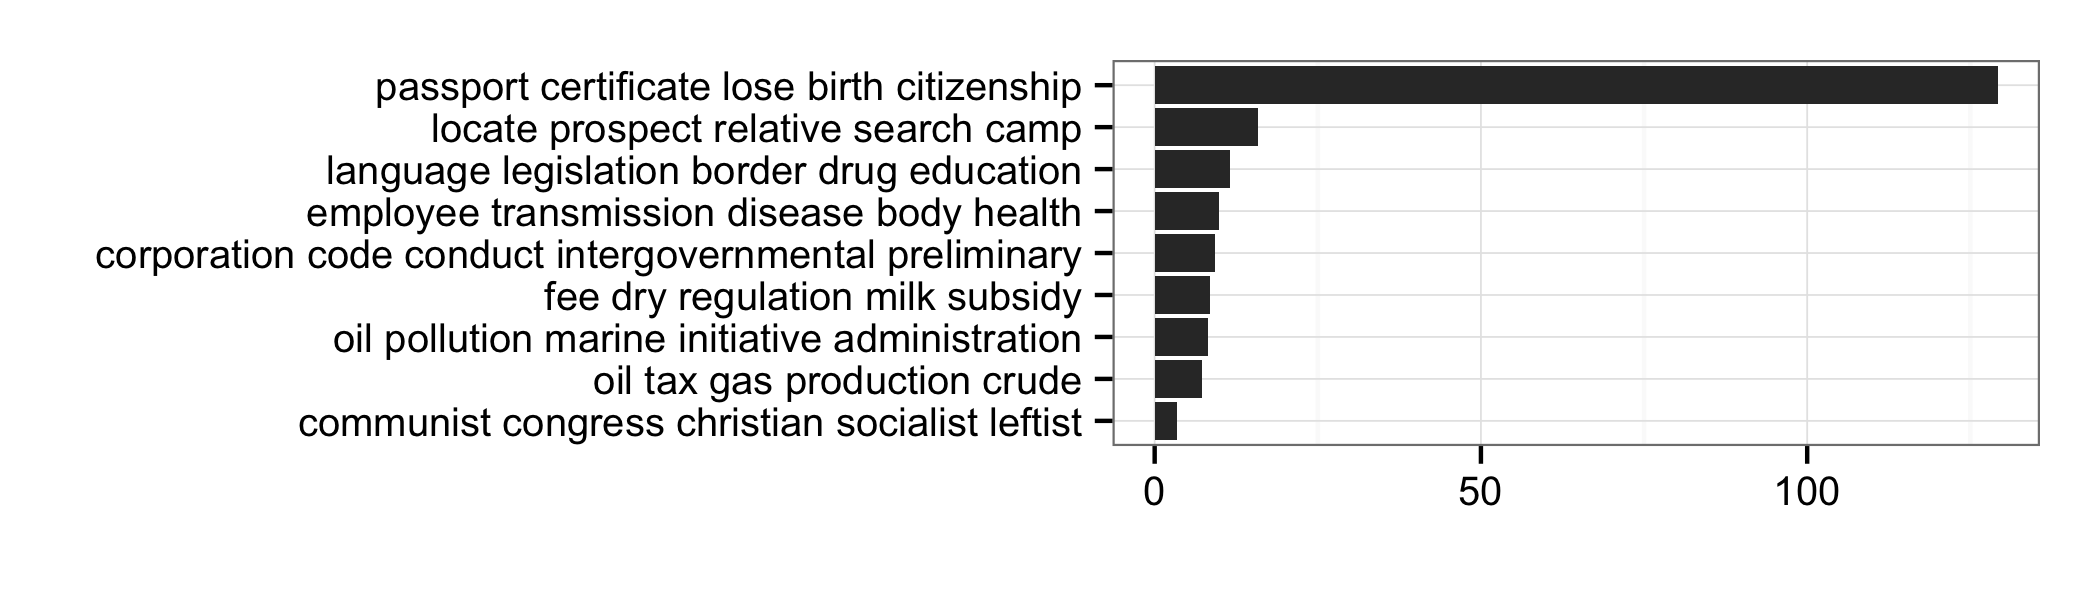
\includegraphics[width=\textwidth]{fig/saigon_topics.png}
\caption{The topics about which the Saigon Embassy usually sends cables.}
\label{fig:saigon_entity}
\end{figure}

Figures~\ref{fig:saigon_march} and~\ref{fig:saigon_april} show two events detected for Saigon in the spring of 1975, just prior to the Fall of Saigon.  Both of these events intuitively match our understanding of true events that occurred during these time periods.

\begin{figure}[ht]
\centering
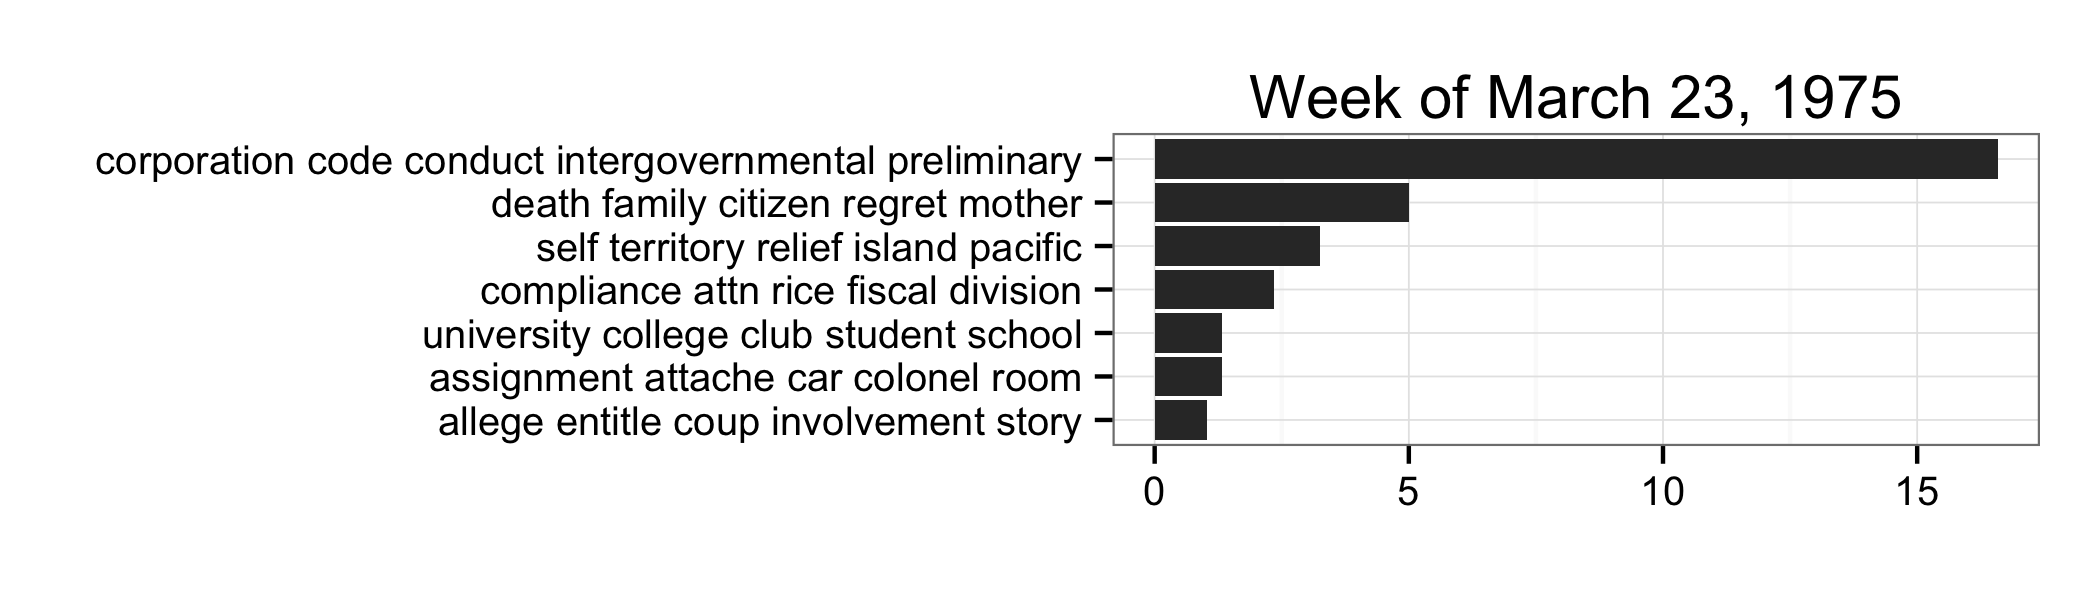
\includegraphics[width=\textwidth]{fig/saigon_march23.png}
\caption{Topical description of the event the week of March 23, 1975.  Advances in March indicated that the city of Saigon would be attacked---the evacuation of American families began at the end of the month.}
\label{fig:saigon_march}
\end{figure}

\begin{figure}[ht]
\centering
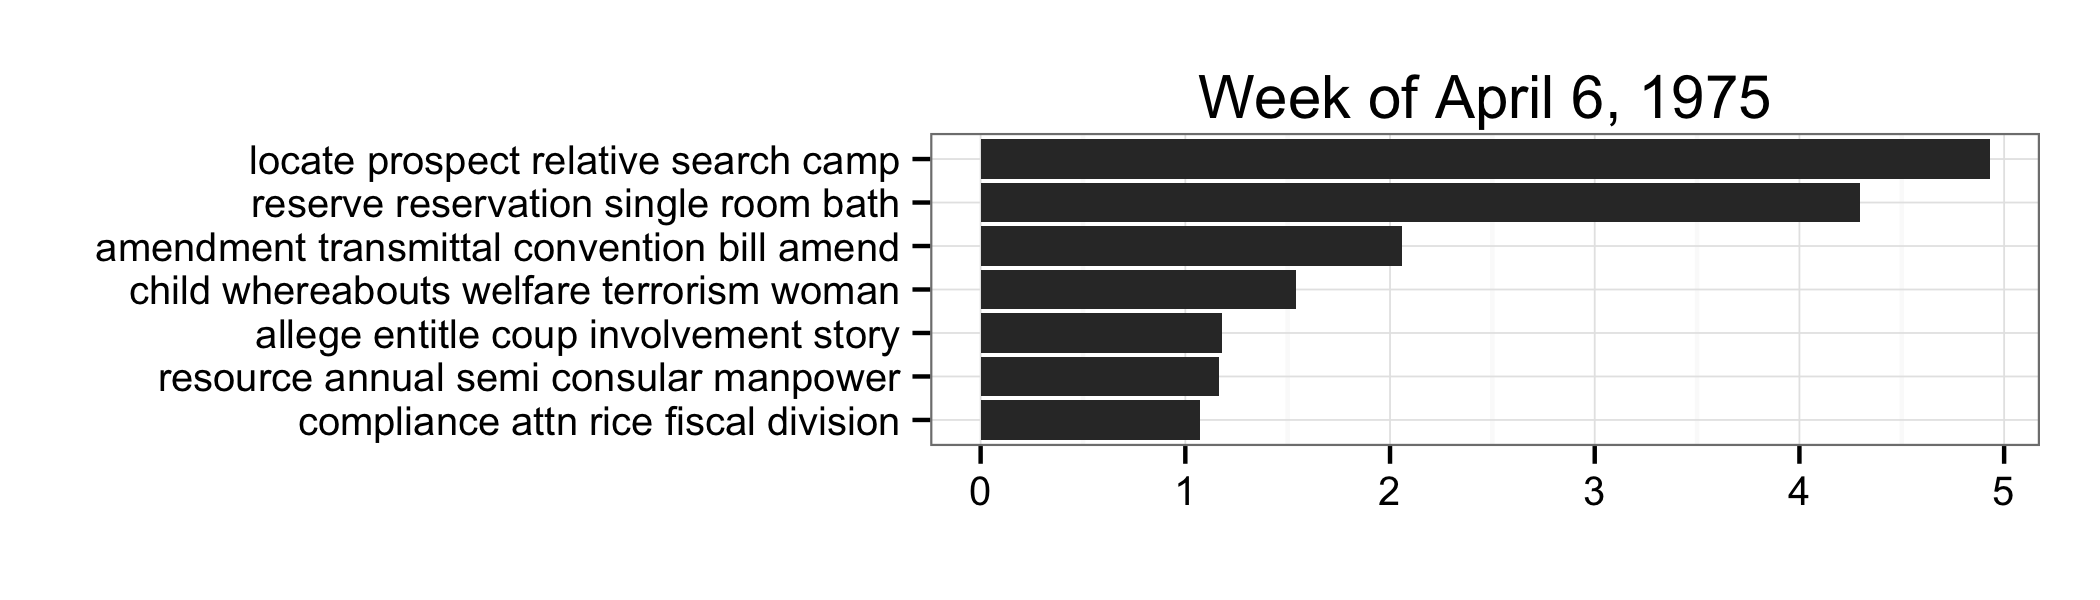
\includegraphics[width=\textwidth]{fig/saigon_apr6.png}
\caption{Topical description of the event the week of April 6, 1975.  During April of this year, lost individuals were being tracked down and children were evacuated in mass from South Vietnam. (See also Figure~\ref{fig:cables_example})}
\label{fig:saigon_april}
\end{figure}

\paragraph{Future Work}  The model we have presented fits each entity independently. In this scenario, modeling ``business-as-usual'' and event topics is more challenging for entities with sparser sending patterns.
We plan to expand our model to include interactions between entities---the State Department will probably interact differently with Moscow than it does with Paris.
Modeling multiple entities interacting with each other about the same topics should make inference easier with regard to describing shared events and ``business-as-usual'' topics.  We also plan to include geographic proximity, which should have a similar effect.

\paragraph{Conclusions} Traditional topic models can describe documents, but they cannot identify when events occur---only a model like ours that explicitly models event occurrences and event content can attribute document observations to discrete events.  Further, by modeling entities, we can distinguish between ``business-as-usual'' document content and content that is attached to particular events---we are also unable to capture this phenomenon with traditional topic models.




\bibliographystyle{apa}
\bibliography{/Users/ajbc/Dropbox/papers/library.bib}


\newpage
\appendix
\section{Inference Details}
\label{sec:appendix_inference}
For now, we assume that we know the LDA topics $\beta$ and only observe the documents in terms of their topics $\theta$; breaking this assumption makes inference a little more complicated as the updates for $\theta$ would have new dependencies.

Variational inference approaches the problem of posterior inference by minimizing the KL divergence from an approximating distribution $q$ to the true posterior $p$.
This is equivalent to maximizing the ELBO: \[\mathcal{L}(q)  = \E_{q(\epsilon, \pi, \phi)}[\log p(\theta,\epsilon,\pi,\phi) - \log q(\epsilon, \pi, \phi)].\]

We define the approximating distribution $q$ using the mean field assumption: \[q(\epsilon, \pi, \phi) = \prod_i q(\epsilon_{i})\prod_k\left[q(\phi_{0k})\prod_i q(\pi_{ik})\right].\]
The variational distributions $q(\pi)$ and $q(\phi)$ are both gamma-distributed with free variational parameters $\lambda^\pi$ and $\lambda^\phi$, respectively.  Because these parameters are free, we use the softmax function $\mathcal{M}(x) = \log(1+\exp(x))$ to constrain them so that they do not violate the requirements of the gamma distribution.
The variational distribution $q(\epsilon)$ is Poisson-distributed with variational parameter $\lambda^\epsilon$; this free parameter is also constrained by the softmax function.

The expectations under $q$, which are needed to maximize the ELBO, do not have a simple analytic form, so we use ``black box'' VI techniques.
F or each variable, we can write the log probability of all terms containing that variable, giving us 
\[\log p^\epsilon_{i}(\theta, \epsilon, \pi, \phi) \triangleq \log p(\epsilon_{i} \g \eta_\epsilon) + \sum_{j : f(a_i, c_j) \neq 0}\sum_k\log p(\theta_{jk} \g \phi_{0k}, c_j, a_i, d, \beta_c, \pi_{ik}, \epsilon_i),\]
\[\log p^\pi_{ik}(\theta, \epsilon, \pi, \phi) \triangleq \log p(\pi_{ik} \g \alpha_0, \beta_0) + \mathbf{1}[\epsilon_i \neq 0] \sum_{j : f(a_i, c_j) \neq 0}\log p(\theta_{jk} \g \phi_{0k}, c_j, a_i, d, \beta_c, \pi_{ik}, \epsilon_i),\]
and
\[p^\phi_{k}(\theta, \epsilon, \pi, \phi) \triangleq \log p(\phi_{0k} \g \alpha, \beta) + \sum_{j} \log p(\theta_{jk} \g \phi_{0k}, c_j, a_i d, \beta_c, \pi_{ik}, \epsilon_i).\]
Then we can write the gradients with respect to the variational parameters as:
\[\nabla_{\lambda^\epsilon_{i}} \mathcal{L} = \E_q \left[ \nabla_{\lambda^\epsilon_{i}} \log q(\epsilon_{i} \g \lambda^\epsilon_{i}) \left( \log p^\epsilon_{i}(\theta, \epsilon, \pi, \phi) - \log q(\epsilon_{i} \g \lambda^\epsilon_{i}) \right)\right],\]
\[\nabla_{\lambda^\pi_{ik}} \mathcal{L} = \E_q \left[ \nabla_{\lambda^\pi_{ik}} \log q(\pi_{ik} \g \lambda^\pi_{ik}) \left( \log p^\pi_{ik}(\theta, \epsilon, \pi, \phi) - \log q(\pi_{ik} \g \lambda^\pi_{ik}) \right)\right],\]
and
\[\nabla_{\lambda^\phi_{k}} \mathcal{L} = \E_q \left[ \nabla_{\lambda^\phi_{k}} \log q(\phi_{0k} \g \lambda^\phi_{k}) \left( \log p^\phi_{k}(\theta, \epsilon, \pi, \phi) - \log q(\phi_{0k} \g \lambda^\phi_{k}) \right)\right].\]

Using this framework, we construct our black box algorithm below in Algorithm 1.

\paragraph{For Reference}
The gamma distribution and derivatives:
\begin{align}
\log\mbox{Gamma}(x \g a,b) & = ab\log b - \log\Gamma \left(ab\right) +(ab-1)\log x - bx \label{eq:gamma}\\
%\log\mbox{Gamma}(x \g \mathcal{M}(a), \mathcal{M}(b)) & = 
%\mathcal{M}(a)\mathcal{M}(b)\log \mathcal{M}(b) - \log\Gamma \left(\mathcal{M}(a)\mathcal{M}(b)\right) +(\mathcal{M}(a)\mathcal{M}(b)-1)\log x - \mathcal{M}(b)x \\
\nabla_a \log\mbox{Gamma}(x \g \mathcal{M}(a), \mathcal{M}(b)) &= 
\mathcal{M}'(a) \mathcal{M}(b) \left[ \log \mathcal{M}(b) - \Psi \left(\mathcal{M}(a)\mathcal{M}(b)\right) + \log x\right] \label{eq:dgammaA}
\\
\nabla_b \log\mbox{Gamma}(x \g \mathcal{M}(a), \mathcal{M}(b)) &= 
\mathcal{M}'(b) \left[ \mathcal{M}(a) \left((\log \mathcal{M}(b) + 1) - \Psi \left(\mathcal{M}(a)\mathcal{M}(b)\right) + \log x\right) - x\right]\label{eq:dgammaB}
%\frac{d}{d b}\log\mbox{Gamma}(x \g \mathcal{M}(a), \mathcal{M}(b)) &= 
%\mathcal{M}'(b) \left[ \mathcal{M}(a) (\log \mathcal{M}(b) + 1) - \mathcal{M}(a)\Psi \left(\mathcal{M}(a)\mathcal{M}(b)\right) + \mathcal{M}(a)\log x - x\right]
\end{align}

The Poisson distribution and derivative:
\begin{align}
\log\mbox{Poisson}(x~\vert~\lambda) &= x\log\lambda - \log(x!) - \lambda \label{eq:poisson} \\
%\log\mbox{Poisson}(x~\vert~\mathcal{M}(\lambda)) &= x\log\mathcal{M}(\lambda) - \log(x!) -\mathcal{M}(\lambda) \\
\nabla_\lambda \log\mbox{Poisson}(x~\vert~\mathcal{M}(\lambda)) &= \mathcal{M}'(\lambda)\left[\frac{x}{\mathcal{M}(\lambda)} -1\right].\label{eq:dpoisson}
\end{align}

The softmax function and derivative:
\[\mathcal{M}(x) = \log(1+e^x)\]
\[\mathcal{M}'(x) = \frac{e^x}{1+e^x}\]
%\SetCommentSty{mycommfont}


\begin{algorithm}
\small
\DontPrintSemicolon
\KwIn{document topics $\theta$}
\KwOut{estimates of latent parameters entity topics $\phi$, event topics $\pi$,
and event occurrences $\epsilon$}
\textbf{Initialize} $\lambda^\pi$, $\lambda^\phi$, and $\lambda^\epsilon$ to
respective priors \;
\textbf{Initialize} iteration count $t = 0$ \;
\While {change in validation likelihood $< \delta$}{
	initialize $\sigma^\pi = 0$ \;
	\For {each sample $s = 1, \dots, S$}{
		\For {each component $k$} {
			draw sample entity topics $\phi_{0k}[s] \sim \mbox{Gamma}(\mathcal{M}(\lambda^\phi_{k}))$ \;
			\BlankLine
			set $p^\phi_k[s] = \log p(\phi_{0k}[s] \g \alpha, \beta)$ \tcp*{see Eqn.~\ref{eq:gamma}}
			set $q^\phi_k[s] = \log q(\phi_{0k}[s] \g \lambda^\phi_k)$ \tcp*{Eqn.~\ref{eq:gamma} with params $\mathcal{M}(\lambda^{\phi}_k)$}
			set $g^\phi_k[s] = \nabla_{\lambda^\phi_{k}} \log q(\phi_{0k}[s] \g \lambda^\phi_{k})$ \tcp*{see Eqns.~\ref{eq:dgammaA}, \ref{eq:dgammaB}}
		}
		\For {each timestep $i$} {
			draw sample event occurance $\epsilon_i[s] \sim \mbox{Poisson}(\mathcal{M}(\lambda^\epsilon_i))$ \;
			\BlankLine
			set $p^\epsilon_i[s] = \log p(\epsilon_{i}[s] \g \eta)$ \tcp*{see Eqn.~\ref{eq:poisson}}
			set $q^\epsilon_i[s] = \log q(\epsilon_i[s] \g \lambda^\epsilon_i)$ \tcp*{Eqn.~\ref{eq:poisson} with param $\mathcal{M}(\lambda^{\epsilon}_i)$}
			set $g^\pi_{i}[s] = \nabla_{\lambda^\epsilon_{i}} \log q(\epsilon_{i}[s] \g \lambda^\epsilon_{i})$ \tcp*{see Eqn.~\ref{eq:dpoisson}}
			\BlankLine
			\If {$\epsilon_i[s] \neq 0$} {
				\For {each component $k$} {
					draw sample event topics $\pi_{ik}[s] \sim \mbox{Gamma}(\mathcal{M}(\lambda^\pi_{ik}))$ \;
					\BlankLine
					set $p^\pi_{ik}[s] = \log p(\pi_{ik}[s] \g \alpha_0, \beta_0)$ \tcp*{see Eqn.~\ref{eq:gamma}}
					set $q^\pi_{ik}[s] = \log q(\pi_{ik}[s] \g \lambda^\pi_{ik})$ \tcp*{Eqn.~\ref{eq:gamma} with params $\mathcal{M}(\lambda^{\pi}_{ik})$}
					set $g^\pi_{ik}[s] = \nabla_{\lambda^\pi_{ik}} \log q(\pi_{ik}[s] \g \lambda^\pi_{ik})$ \tcp*{see Eqns.~\ref{eq:dgammaA}, \ref{eq:dgammaB}}
				}
			}
		}
	}
	
	\For {each document $j$ (sent on date $c_j$ and has topics $\theta_j$), sample $s$ and component $k$}{
		set $\phi_{jk}[s] = \phi_j[s] + \sum_i f(a_i, c_j) \epsilon_i[s] \pi_{ik}[s]$ \;
		set $p^\theta_{jk}[s] = \log p(\theta_{jk} \g \phi_{jk}[s], \beta_c)$ \tcp*{see Eqn.~\ref{eq:gamma}}
		\BlankLine
		$p^\phi_k[s] \pluseq p^\theta_{jk}[s]$ \;
		\For {each timestep $i$ where $a_i \le c_j < a_i + d$}{
			$p^\epsilon_{i}[s] \pluseq \sum_k p^\theta_{jk}[s]$ \;
			\If {$\epsilon_i[s] \neq 0$} {
				$p^\pi_{ik}[s] \pluseq p^\theta_{jk}[s]$ \;
				update $\sigma^\pi_i \pluseq 1$ \;
			}
		}
	}

	
	set $\hat\nabla_{\lambda^{\phi} }\mathcal{L} \triangleq \frac{1}{S} \sum_s g^\phi[s] ( p^\phi[s] -  q^\phi[s] )$ \;
	set $\hat\nabla_{\lambda^{\epsilon}} \mathcal{L} \triangleq \frac{1}{S} \sum_s g^\epsilon[s] ( p^\epsilon[s] -  q^\epsilon[s] )$ \;
	set $\hat\nabla_{\lambda^{\pi}} \mathcal{L} \triangleq \frac{1}{\sigma_\pi} \sum_s g^\pi[s] ( p^\pi[s] -  q^\pi[s] )$ \;

	\BlankLine
	set $\rho= (t +\tau)^\kappa$ \;
	% update event content for each event $i$ and topic $k$: 
	set $\lambda^{\pi} \pluseq \rho \hat\nabla_{\lambda^{\pi}} \mathcal{L}$ \;
	set $\lambda^{\epsilon} \pluseq \rho \hat\nabla_{\lambda^{\epsilon}} \mathcal{L}$ \;
	set $\lambda^{\phi} \pluseq \rho \hat\nabla_{\lambda^{\phi}} \mathcal{L}$ \;
}

set $\E[\pi] = \lambda^{\pi,a}$ \;
set $\E[\phi] = \lambda^{\phi,a}$ \;
set $\E[\epsilon] = \lambda^{\epsilon}$ \;
\BlankLine
\Return{$\E[\pi]$, $\E[\phi]$, $\E[\epsilon]$} \;
\caption{Inference for Cables Model}
\label{alg:cables}
\end{algorithm}

\paragraph{Validation of Implementation}
To show that our algorithm fits our model appropriately, Figure~\ref{fig:ELBO} shows that the ELBO is maximized.  While the ELBO does decrease slowly after reaching a local maximum, this sort of over-fitting can be avoided with an appropriate convergence metric, like considering the change in data likelihood. Using this as a metric, the shown ELBO would have converged around iteration 10.
\begin{figure}[ht]
\centering
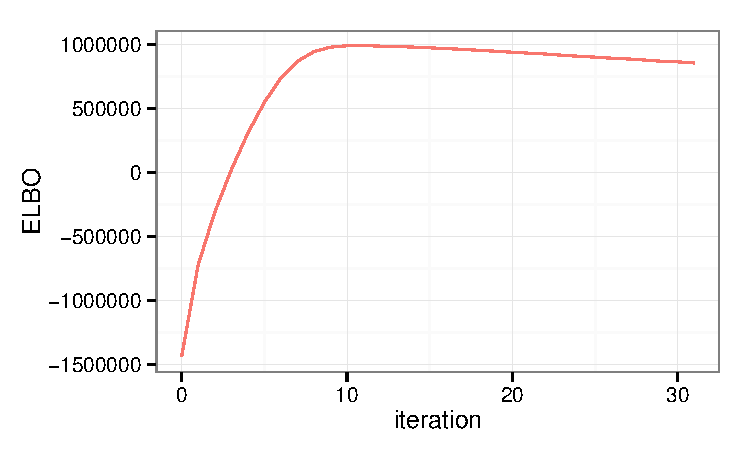
\includegraphics[width=0.7\textwidth]{fig/ELBO.pdf}
\caption{The ELBO on a small collection of documents.}
\label{fig:ELBO}
\end{figure}


\end{document}
